\documentclass{hbrs-ecta-report}

\usepackage{float}
\usepackage{placeins}
\usepackage{ngerman}
%\usepackage[utf8]{inputenc}
\usepackage{fontspec}
\begin{document}

\conferenceinfo{H-BRS}{2017}

\title{Neuroevolution: Backpropagation}
\subtitle{}

\numberofauthors{2}
\author{
\alignauthor
Tim L"ugger, Jan Urfei
}

\date{today}
\maketitle
\begin{abstract}
Aufgabe: Approximieren Sie Island mit einem neuronalen Netz und stellen Sie die Approximation graphisch dar. Stellen Sie den Verlauf des Fehlers über die Zeit für alle drei Sets dar und veranschaulichen Sie den Einfluss unterschiedlicher Lernraten auf den Lernprozess.
\end{abstract}

\section{Backpropagation}
\paragraph{Neuronales Netz}
Grundlage für Backpropagation ist ein neuronales Netz (siehe Figure \ref{fig:neuronalesNetz}). Ein Neuronales Netz besteht aus mehreren Neuronen, die in verschiedenen Schichten (Layern) angeordnet sind. Es wird generell zwischen dem ''input Layer'', den ''hidden Layer'' und dem ''output Layer'' unterschieden. Dabei besteht der input Layer aus den Neuronen die eine Eingabe in das Netz bekommen. Der Output Layer liefert nachher die Ergebnisse des Neuronalen Netzes. Alle Neuronen zwischen input und output Layer liegen auf den hidden Layern, welche beliebig viele sein können. Die Anzahl der Neuronen pro Layer ist auch beliebig. Bei dem Input Layer hängt es von der Eingabe ab und bei dem Output Layer hängt es von dem ab, was man nachher als Ergebnis haben will.\\
Das Neuronale Netz in Figure \ref{fig:neuronalesNetz} besitzt 6 Input Neuronen, 2 Hidden Layer mit jeweils 4/3 Neuronen und ein Output Neuron.
\begin{figure}[h!]
	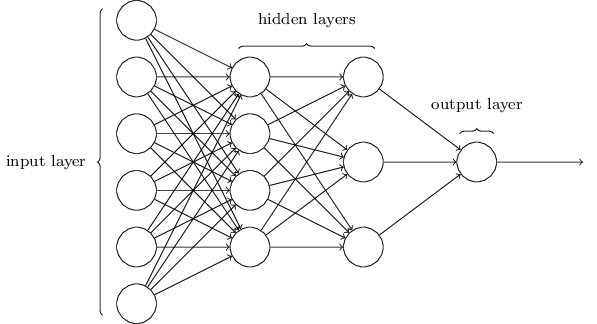
\includegraphics[width=0.6\linewidth]{img/neuronalesNetz}
	\caption{Neuronales Netz mit zwei Hidden Layer}
	\label{fig:neuronalesNetz}
\end{figure}

\FloatBarrier

 \paragraph{Neuron}
 Wie funktioniert ein Neuron? Ein Neuron kann mehrere Eingaben haben( Figure \ref{fig:Neuron}). Bei den Input Neuronen kommt diese Eingabe von außen, bei allen anderen kommt die Eingabe von dem Output von anderen Neuronen. Alle Eingaben des Neurons haben ein zugeordnetes Gewicht, welches beim Trainieren angepasst wird, aber dazu später. Alle Eingaben von einem Neuron werden jetzt gewichtet Aufsummiert und bilden die Netzeingabe für das eine Neuron. Allgemein muss noch eine Aktivierungsfunktion für alle Neuronen definiert werden, die ein Neuron erst ab einer gewissen Eingabe ''aktiv'' werfen lässt. Die Netzeingabe eines Neuron wird also in die Aktivierungsfunktion gegeben und bildet dann den Output eines Neurons.
 
\begin{figure}[h!]
	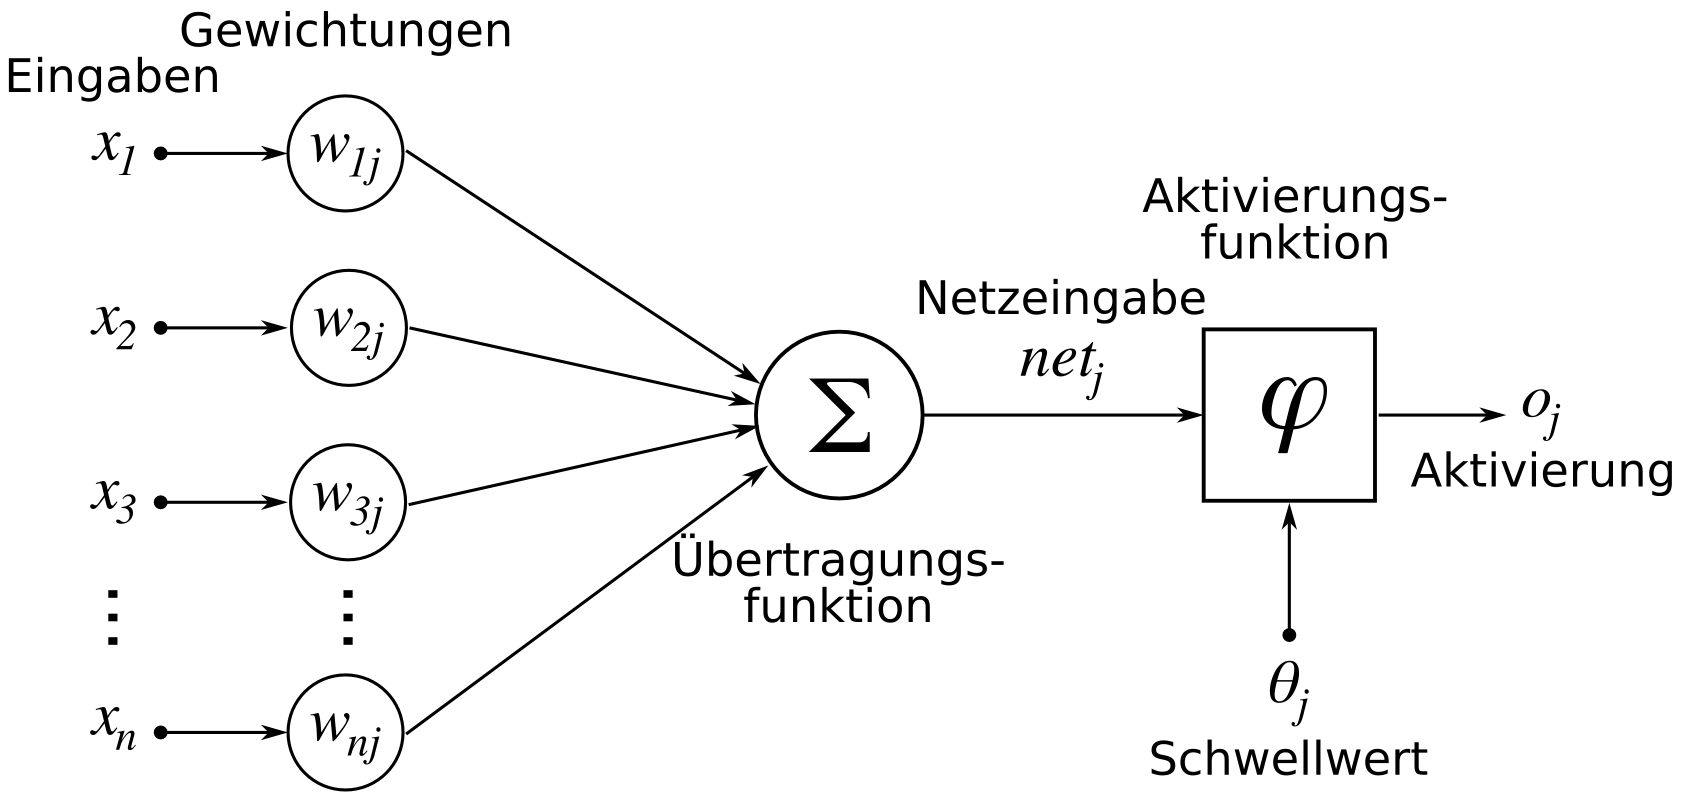
\includegraphics[width=\linewidth]{img/Neuron}
	\caption{Ein Neuron}
	\label{fig:Neuron}
\end{figure}

\paragraph{Backpropagation}
Backpropagation besteht aus mehreren Phasen. Zu Erst gibt es einen sogenannten ''Forward Pass''. Dabei wird ein Wert von der Trainingsmenge in das Neuronale Netz (am Input Layer) gegeben. Es wird für jedes Layer der Output mit den aktuellen Kantengewichten berechnet. Den Output vergleicht man dann mit den Soll Wert und bildet daraus den Fehler der zwischen Output und Soll besteht. Für die Berechnung dieses Fehlers gibt es unterschiedliche Verfahren. \\
Wenn der Fehler feststeht wird geguckt, wie sich das Ergebnis von dem vorherigen Layer zusammengesetzt hat. Es wird mathematisch gesehen der größte Gradient bestimmt. Da man bei minimal kleinen Schritten davon ausgehen kann, dass in entgegengesetzter Richtung der kleinste Gradient liegt, passt man die Kantengewichte in Richtung des negativen Gradient mit einer festgelegten Lernrate an. So geht man von Schicht zu Schicht rückwärts, bis man beim Input Layer angekommen ist.
Wenn das der Fall ist nimmt man sich den nächsten Trainingsdatensatz und beginnt wieder von vorne. Mit dem gesamten Trainingsdatensatz trainiert man immer wieder das Neuronale Netz, bis der Fehler klein genug ist. Allerdings sollte man die Reihenfolge der Trainingsdaten zwischen den Durchläufen ändern, da das Neuronale Netz sonst auch die Reihenfolge von den Trainingsdaten lernt, was einen negativen Einfluss auf andere Daten haben kann, für die man das Netz vielleicht später verwenden will.


\section{Herangehensweise}
 Zuerst werden alle Höhen Daten von Island (Figure \ref{fig:island}) aufgeteilt in drei Zufällig gewählte Mengen. Dabei entsprechen 70\% aller Daten derer, die für das trainieren des Neuronalen Netzes verwendet werden. Jeweils 15\% werden dafür verwendet, um das Ergebnis zu validieren und zu testen. 
\begin{figure}[h!]
	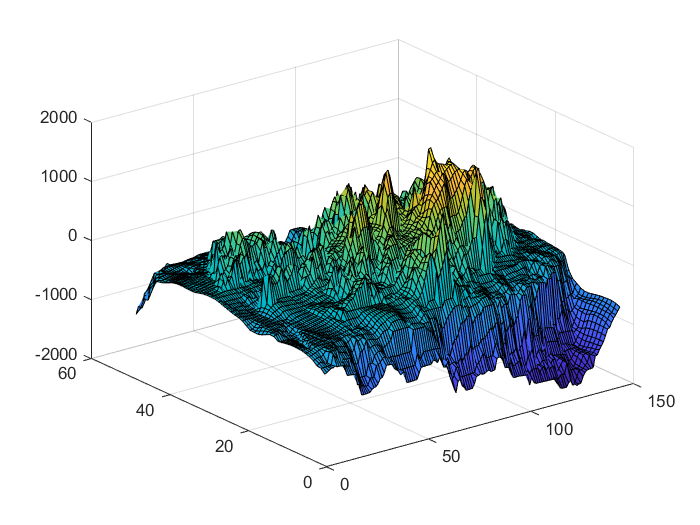
\includegraphics[width=\linewidth]{img/island}
	\caption{Höhenprofil von Island}
	\label{fig:island}
\end{figure}

Unsere Netztopologie sieht im Moment so aus, dass wir zwei Neuronen auf dem Input Layer haben, die mit den X und Y Koordinaten gefüttert werden. Nach dem Input Layer haben wir ein Hidden Layer mit 20 Neuronen. Unser Output Layer besitzt nur ein Neuron, da unsere Neuronales Netz ja die Höhe von einem gewissen Punkt auf Island vorhersagen soll.
Für den Vorwärtspass verwenden wir aktuell folgende Funktion als Aktivierungsfunktion: $\frac{1}{1+e^{-x}}$ .\\
Da uns diese Funktion nur Werte zwischen -1 und 1 wiedergibt müssen wir unsere Höhen werte noch normalisieren. Das haben wir gemacht, indem wir jeden Wert durch das Maximum des Betrages der Höhe ($ |max(Hoehe)| $) dividieren.\\
Als Fehler, den wir minimieren wollen verwenden wir den summed squared Error ( $ 0.5*(Soll-Output)^2 $). Wir lassen den Trainingsdatensatz eine X mal wiederholen, bis das trainiert ist. Aktuell haben wir X auf 1000 gesetzt. Nach jedem Durchlauf werden die Trainingsdaten neu angeordnet, damit die Reihenfolge der Trainingsdaten nicht das Ergebnis beeinflussen.

\section{Unsere Ergebnisse}

Es wurden manuell einige Experimente durchgeführt. Ein gutes Ergebnis ist hier dargestellt.
Auf der X-Achse stellt eine Einheit eine komplette Iteration durch die Trainingsdaten dar. Auf der Y-Achse ist dazu jeweils der aktuelle Fehler dargestellt. \newline
Man erkennt, dass sich der Fehler in den ersten Iterationen stark reduziert und danach abflacht. Weitere Trainingsiterationen tragen dann nur noch zu geringfügig zur Reduzierung des Fehler bei.

Entscheidend für das Training ist die zum einen die zufälliger Initialisierung der Gewichtsmatrizen die vor- oder nachteilige Startwerte verursachen kann und zum anderen die gewählte Lernrate. Ist Lernrate zu groß, verändern sich die Gewichte für jedes Trainingsbeispiel zu stark und es findet keine oder nur sehr schlechte Approximation statt. Wird hingegen die Lernrate zu gering gewählt, dauert das Training wesentlich länger, da für nennenswerte Änderungen der Gewichte viel mehr Iterationen benötigt werden.   

\begin{figure}[h]
	\centering
	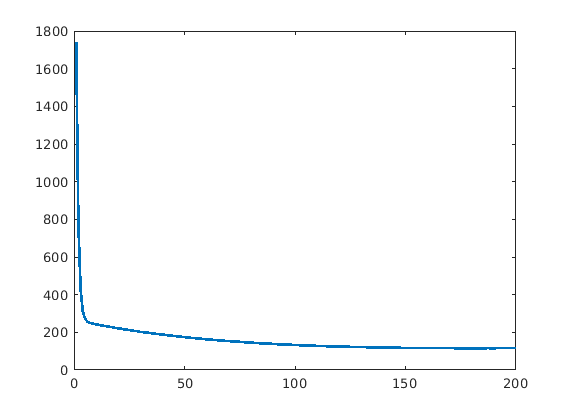
\includegraphics[width=\linewidth]{img/trainingError}
	\caption{Training Set Error, auf diesen Daten wurde trainiert}
	\label{fig:trainingerror}
\end{figure}

\begin{figure}[h]
	\centering
	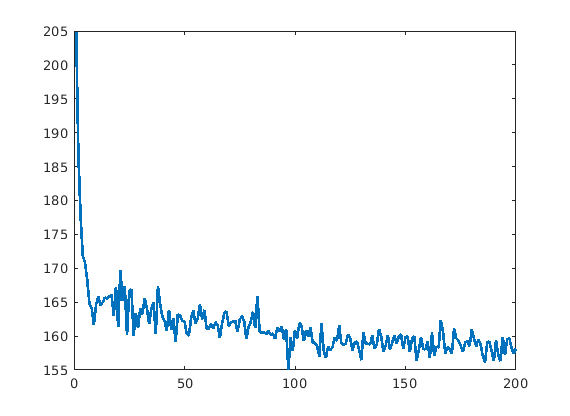
\includegraphics[width=\linewidth]{img/validationError}
	\caption{Validation Set Error: Mit Hilfe dieser Daten werden die Hyperparameter angepasst }
	\label{fig:validationerror}
\end{figure}

\newpage

\begin{figure}[h]
	\centering
	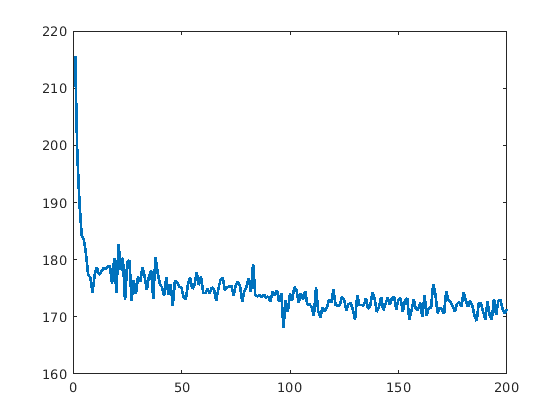
\includegraphics[width=\linewidth]{img/testError}
	\caption{Test Set Error: Auf diesen Daten wird die anschließende Güte der Approximation beurteilt}
	\label{fig:testerror}
\end{figure}

\begin{figure}[h]
	\centering
	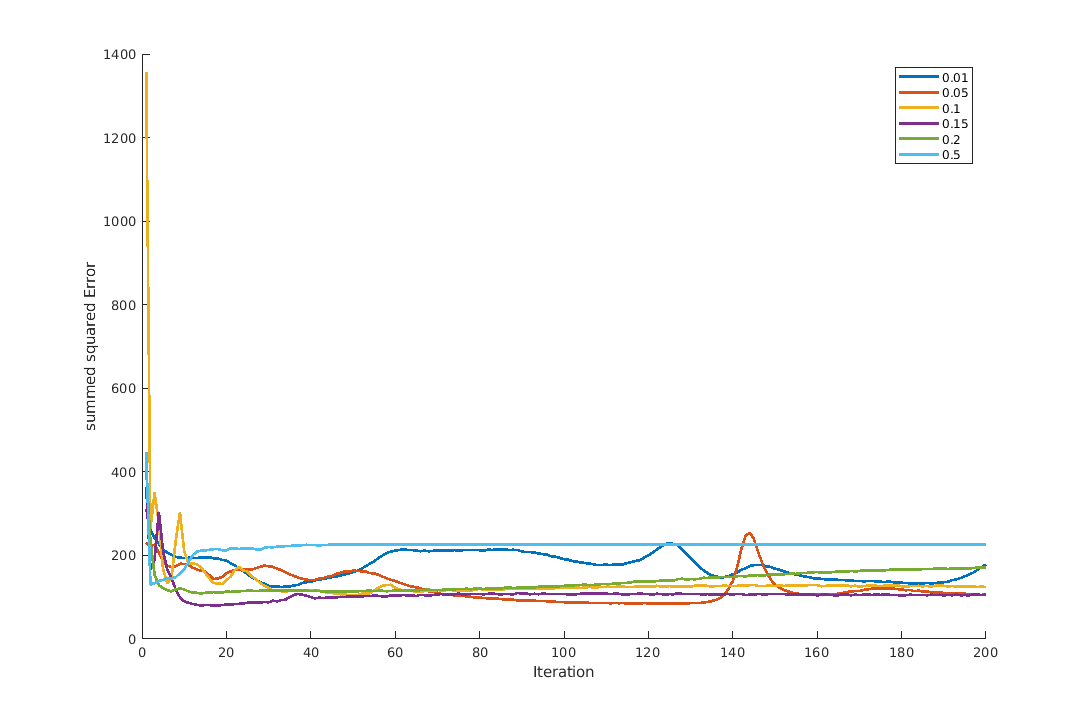
\includegraphics[width=\linewidth]{img/learing_rate_comparison}
	\caption{Vergleich der Lernraten}
	\label{fig:learingratecomparison}
\end{figure}

\FloatBarrier

\subsection{Overfitting}
Bei diesem Experiment wurden zwar ein geringerer Fehler (ca. 87) auf dem Trainingsdaten erreicht der Fehler auf den Validierungsdaten hat sich auch im laufe des Trainings leicht verringert, ist aber nach über 200 Iterationen wieder stark gestiegen. (Figure \ref{fig:validationerroroverfitted}) 
Dies lässt dadurch erklären, dass sich das Netz zu stark an die Trainingsdaten angepasst hat und daher keine Generalisierung möglich ist.

\begin{figure}[ht!]
	\centering
	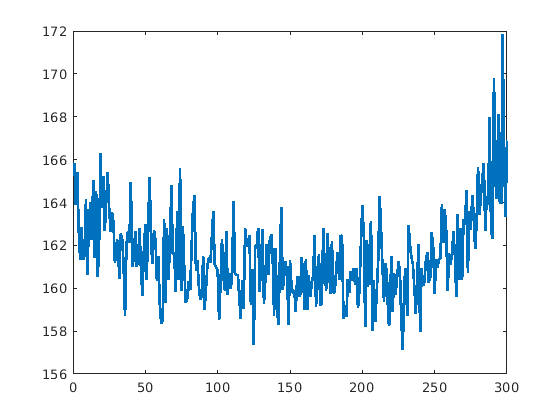
\includegraphics[width=\linewidth]{img/validationErrorOverfitted}
	\caption{Validation Set Error: Bei Overfitted Testset}
	\label{fig:validationerroroverfitted}
\end{figure}



\end{document}
}